\chapter{Einleitung}
Um die Klimaschutzziele zu erreichen, wird eine Vielzahl von Maßnahmen notwendig sein, die nur im Zusammenspiel zum Erfolg führen können. Ein großes Problem bei der Nutzung erneuerbarer Energien ist deren Volatilität, daher sind deutlich größere Speichermöglichkeiten erforderlich. Ein Medium für die langfristige Speicherung und den Transport von Energie bietet Wasserstoff, der auf unterschiedliche Weise gewonnen werden kann und vielfältige Einsatzmöglichkeiten bietet. In der Industrie wird Wasserstoff bereits heute in großem Umfang eingesetzt. In den meisten Fällen wird er jedoch durch Dampfreformierung direkt am Einsatzort aus Erdgas gewonnen. Zukünftig kann er durch den Einsatz von Elektrolysezellen mit erneuerbaren Energien nachhaltig erzeugt werden \cite{Elektrolyse}. 
\section{Stand der Technik}
 Die Entwicklung der Elektrolyse schreitet sehr schnell voran und in den nächsten Jahren sind Veränderungen zu erwarten, die auch die Stromversorgung betreffen. Insbesondere der Trend zu höheren Spannungsklassen ermöglicht eine Kostenreduktion auf Seiten der Leistungselektronik. Die optimale Auslegung der Elektrolyseanlage hängt jedoch von vielen anwendungsspezifischen Parametern wie z.B. der Betriebsführung ab. Insbesondere die Entwicklung des Strompreises und die Netzstabilität in der Zukunft können die Amortisation stark beeinflussen. Durch Gleichrichter, die das Netz unterstützen, anstatt es z.B. durch Blindleistungsbezug zu belasten, können Elektrolyseure ohne zusätzliche Kompensationsanlagen günstiger betrieben werden. Darüber hinaus kann durch Frequenzstabilisierung und andere \gls{SDL} zusätzliche Vergütung generiert werden. \\
Die \gls{IRENA} hat in ihrem Bericht über die Kostenentwicklung der Elektrolyse im Jahr 2020 den Anteil der Kosten für die Stromversorgung für \gls{PEM}-Elektrolyseure mit 29 bis 38 Prozent angegeben. Wobei die Elektrolysezellen selbst weniger als die Hälfte der Kosten ausmachen. Darüber hinaus werden als mögliche Faktoren zur Senkung der Gleichrichterkosten Skaleneffekte, die Standardisierung von Komponenten sowie die Beteiligung von Unternehmen aus der Elektronikindustrie anstelle von Elektrolyseurherstellern genannt \cite{IRENA2020}.\\ 
	\begin{figure} [H]
		\centering
		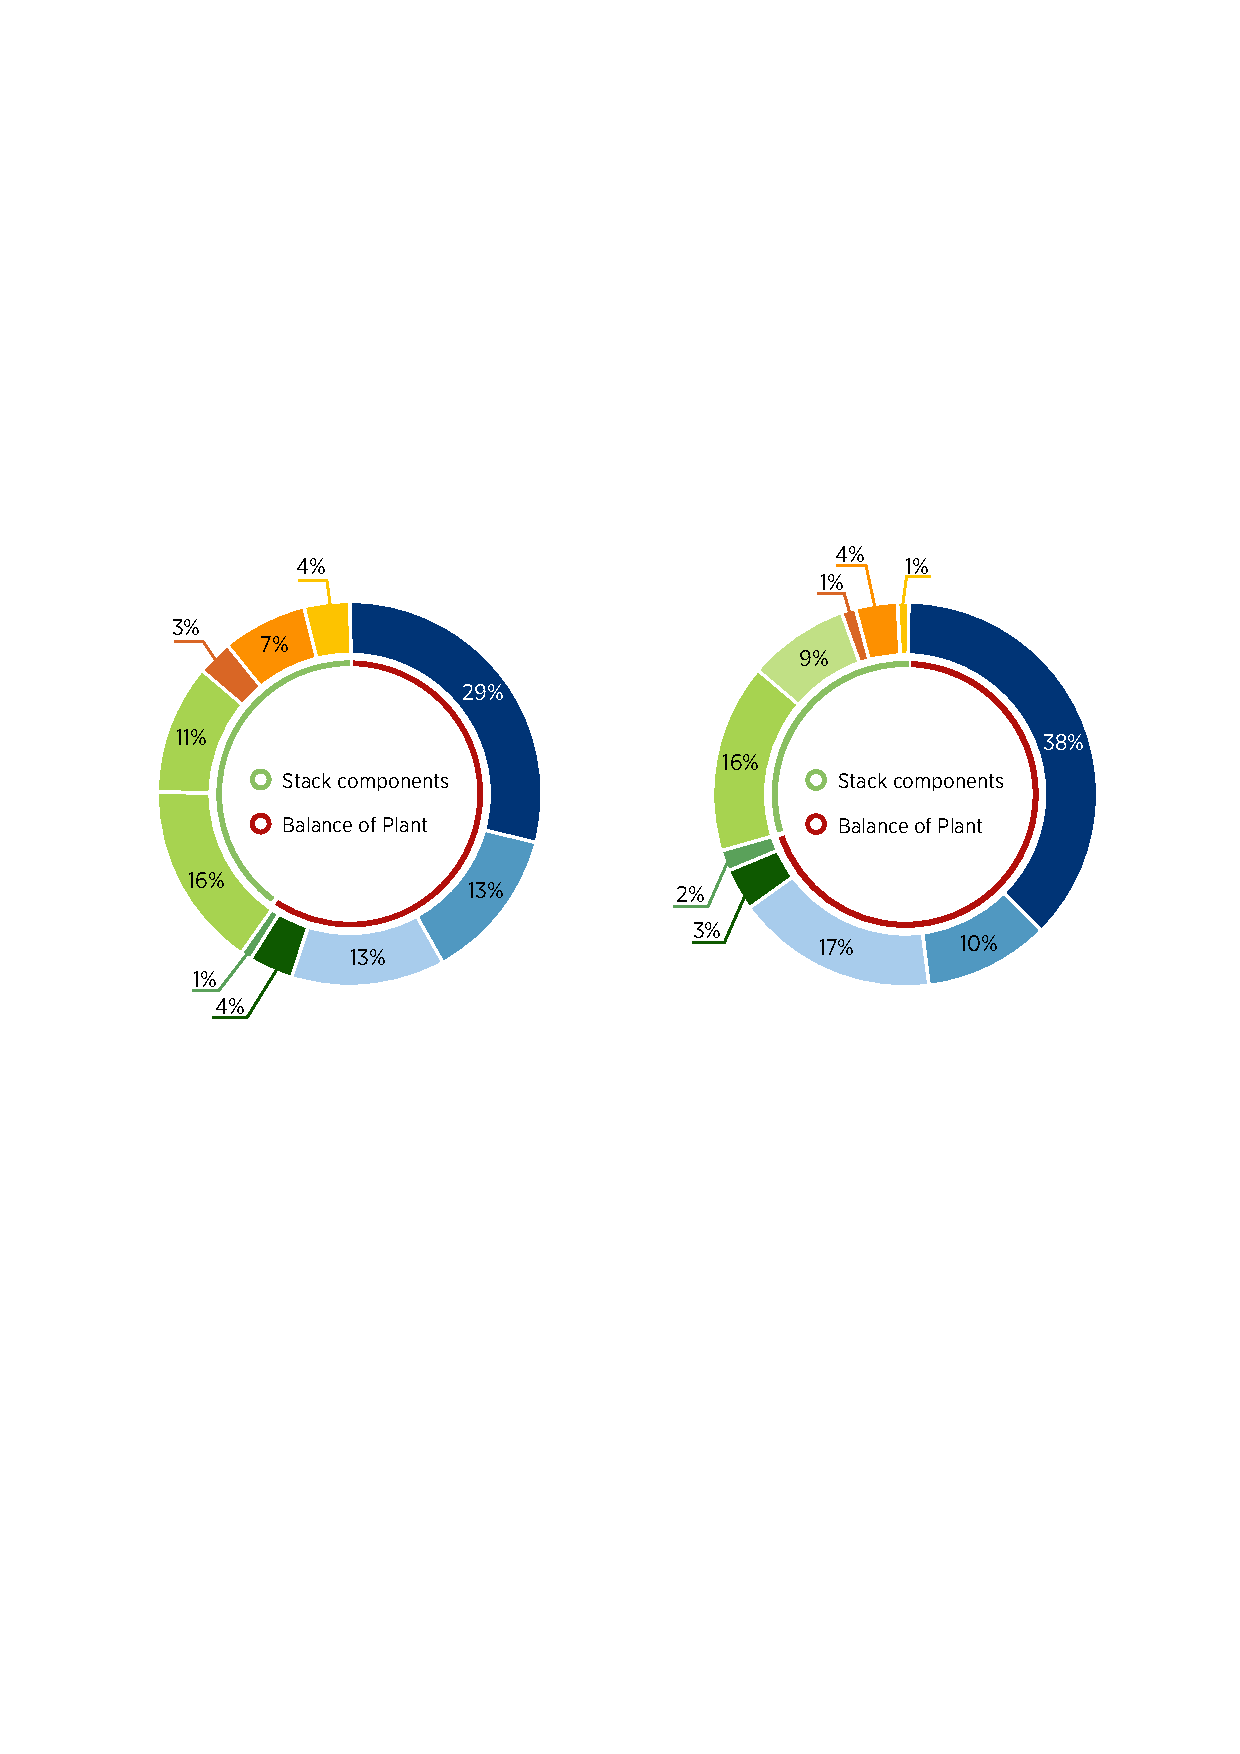
\includegraphics[width=0.7\linewidth]{content/Grafiken/ElyCost}
		\caption[Systemkosten PEM Elektrolyse]{Systemkosten \gls{PEM} Elektrolyse links 10 MW pro Jahr, rechts 1 GW pro Jahr \cite{IRENA2020}}
		\label{fig:elycost}
	\end{figure}
Die Abb. \ref{fig:elycapacity} zeigt zudem, dass der Ausbau der Elektrolyse in den letzten Jahren enorm zugenommen hat und in Zukunft noch deutlich zunehmen wird. Die weltweite Leistung hat gerade den Gigawatt-Bereich erreicht und soll allein in Deutschland bis 2030 auf mindestens zehn Gigawatt ausgebaut werden.\\
	\begin{figure}[H]
		\centering
		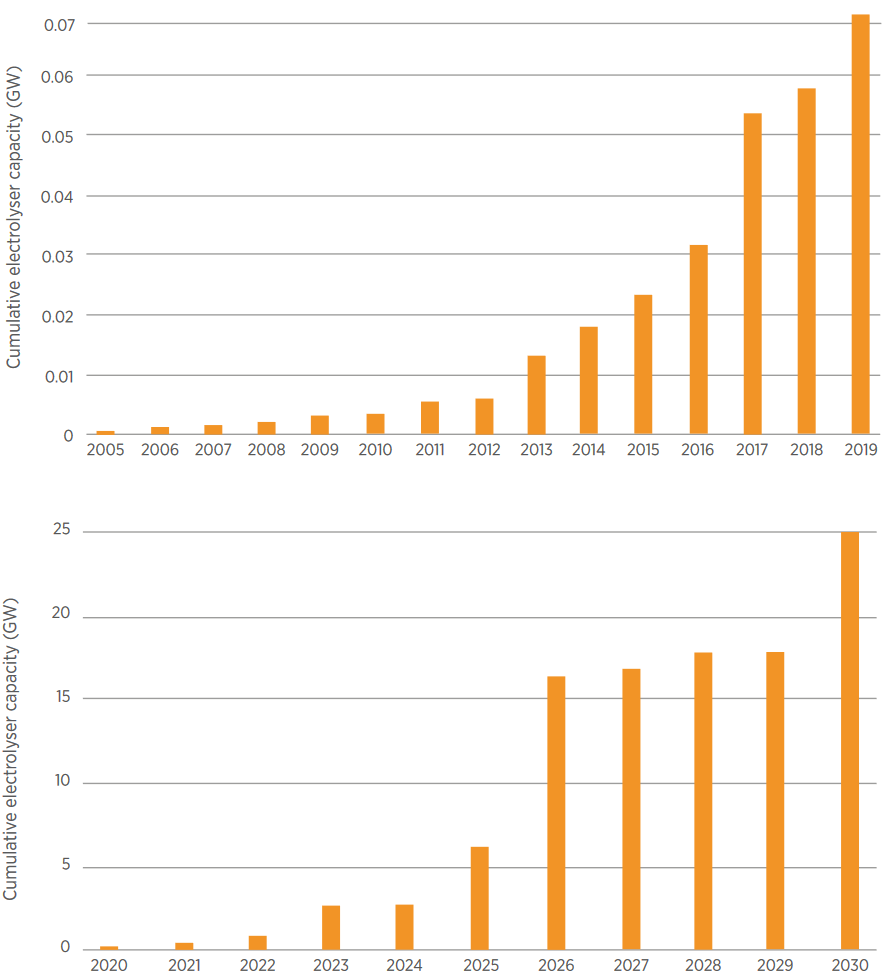
\includegraphics[width=0.7\linewidth]{content/Grafiken/Ely_Capacity}
		\caption[Elektrolyse Kapazität bis 2030]{Elektrolysekapazität Stand 2020 mit Ausblick bis 2030 \cite{IRENA2020}}
		\label{fig:elycapacity}
	\end{figure}
Ein grundlegendes Unterscheidungsmerkmal für Gleichrichterschaltungen ist die Umsetzung als Dioden/Thyristor oder aktiver Gleichrichter. In Abbildung \ref{fig:thyristor} ist ein Beispiel für einen Thyristor-Gleichrichter zu sehen . 
	\begin{figure} [H]
		\centering
		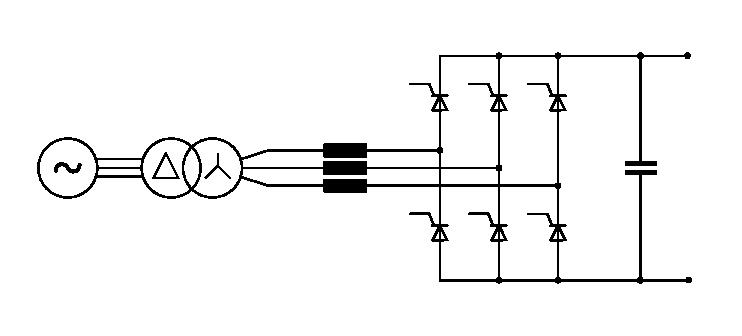
\includegraphics[width=0.9\linewidth]{content/Grafiken/Thyristor}
		\caption{Aufbau eines Thyristor-Gleichrichters}
		\label{fig:thyristor}
	\end{figure}
Thyristorgleichrichter haben aufgrund ihrer kompakten Bauform eine höhere Leistungsdichte und können in großen Stückzahlen kostengünstig produziert werden. Zudem gibt es bereits zahlreiche Lösungen für unterschiedliche Anwendungen. Eine Übersicht mit Bewertung geeigneter Gleichrichter für den Einsatz in Elektrolyseanlagen wurde von Mengxing Chen et al. erstellt \cite{HydrogenElectronicTopologies}. Aktive Gleichrichter zeichnen sich durch ihre Netzqualität aus. Aufgrund seiner Blindleistung benötigt er zusätzliche STATCOM-Anlagen zur Kompensation am Netzanschlusspunkt. Um eine bessere Performance zu ermöglichen, können zusätzlich Zerhacker (Chopper) erforderlich sein. Durch die 12-pulsige Anordnung und die höhere Ausgangsspannung ist der Aufbau des Netztransformators komplexer \cite{HydrogenRectInf}. Aktive Gleichrichter können einen konstanten Leistungsfaktor erreichen und benötigen daher keine Kompensationsanlagen. Außerdem kann die Verzerrung \gls{THD} unter 5 \% liegen, so dass der Filteraufwand geringer ist. Durch Multi-Level-Topologien können Halbleiter besser ausgenutzt und der Wirkungsgrad erhöht werden. Innovative Konzepte erfordern jedoch einen höheren Entwicklungsaufwand und die Zuverlässigkeit ist schwieriger zu gewährleisten. Einen Überblick über die Eigenschaften gibt die Tabelle \ref{tab:thyVSafe}.\\
	\begin{table} [H]
		\centering
		\caption{Vergleich Thyristor-Gleichrichter und aktiver Gleichrichter}
		\label{tab:thyVSafe}
		\begin{tabular}{|c|c|} 
			\hline
			\textbf{Diode / Thyristor} & \textbf{Aktiver Gleichrichter} \\
			\hline
			Hohe Leistungsdichte & Einheitlicher Leistungsfaktor \\
			\hline
			Geringe Halbleiterkosten & <5 \% \gls{THD} \\
			\hline
			Vorgefertigte Lösungen &  \gls{SDL} möglich \\
			\hline
			Benötigt STATCOM & Mehr Level Topologien  \\
			\hline
			Zusätzlicher Zerhacker (Chopper) ggf  nötig & Innovative Lösungen \\
			\hline
			Komplexer Transformator & Aufwändigere Entwicklung \\
			\hline
		\end{tabular}
	\end{table}
Für Gleichrichter im Megawattbereich sind Thyristorschaltungen die am häufigsten verwendete Lösung, da diese Halbleiter aufgrund ihrer langjährigen Entwicklung sehr zuverlässig und robust sind. Zur Optimierung von Blindleistung und \gls{THD} werden meist 12-Puls-Schaltungen verwendet, dies wird durch Verschieben und Überlagern der einzelnen Schaltungen erreicht. Bei Reduzierung der Ausgangsleistung muss jedoch der Zündwinkel so weit vergrößert werden, dass eine externe Blindleistungskompensation erforderlich wird \cite{HydrogenElectronicTopologies}. Daher sind diese Schaltungen nur für Anlagen geeignet, die die meiste Zeit mit hoher Leistung betrieben werden. Ein weiterer Nachteil ist, dass die Elektrolyseure mit gleicher Leistung und Ausgangsspannung betrieben werden müssen. Dadurch ist zum einen eine Wartung an einzelnen Stacks sowie der Austausch einzelner Stacks nicht möglich. Dies stellt bei großen Anlagen ein Problem dar, da die Spannung der Stacks über die Laufzeit ansteigt und ein neuer Stack eine andere Spannung benötigt.\\
Aktuelle Forschungsergebnisse zu Hochleistungsgleichrichtern für die Elektrolyse sind in \cite{HydrogenRectifier} dargestellt. Hier zeigt sich, dass insbesondere bei höheren Ausgangsspannungen neue Konzepte mit integrierter Blindleistungskompensation wie der Vienna-Gleichrichter gut geeignet sind \cite{HydrogenRectifier}.
\pagebreak
\section{Ziel der Arbeit}
Ziel ist es, die beiden ausgewählten Stromrichtertopologien (\gls{IAF} und \gls{B6PFC}) anhand detaillierter Simulationen unter vorgegebenen Randbedingungen zu vergleichen, um eine eindeutige Bewertung vornehmen zu können. Dazu werden zunächst die Randbedingungen der Schnittstellen Elektrolyseur und Stromnetz definiert, um diese in einer Simulation mit Matlab und der Erweiterung PLECS abzubilden. Durch die Modellierung der Halbleiter kann die Verlustleistung und damit der Wirkungsgrad und indirekt der Kühlaufwand abgeschätzt werden. Zusätzlich kann durch die in den magnetischen Komponenten gespeicherte Energie deren Größe und Kosten abgeschätzt werden, da diese den größten Anteil an den Gesamtkosten eines Umrichters ausmachen. Weitere Komponenten wie Treiberschaltungen und benötigte Kapazitäten spielen bei der Bewertung eine untergeordnete Rolle. Um die Bereitstellung von Systemdienstleistungen zu berücksichtigen, wird die Verlustleistung bei einer Phasenverschiebung von 30 Grad und 0 Grad betrachtet. Anschließend erfolgt eine Gesamtbewertung durch Gewichtungsfaktoren der einzelnen Kategorien.